\documentclass{article}
\usepackage[utf8]{inputenc}
\usepackage{titling}
\usepackage{pgfgantt}
\usepackage{graphicx}
\usepackage{pdflscape}
\renewcommand{\refname}{Kaynakça}
\renewcommand{\figurename}{Resim}
\pretitle{
  \begin{center}
  \LARGE\bfseries
  
\includegraphics[width=0.2\textwidth]{ksbu.png} % Başlık önüne ekleyeceğiniz bir logo
  \vskip 1em
}
\title{Reinforcement Learning ile Yapay Zekaya Hayatta Kalmayı Öğretme}
\author{Hüseyin Buğra Taştan}
\date{Mart 2024}

\begin{document}

    \maketitle
    \begin{center}
        
\includegraphics[width=0.4\textwidth]{forest.jpg} 
    \end{center}
    \vfill
    \rule{\textwidth}{0.5pt}
    \renewcommand{\abstractname}{Özet}
\begin{abstract}
\noindent "AI Learns To Survive" adlı proje, derin güçlendirme öğrenme (deep reinforcement learning) kullanarak yapay zeka ajanlarının hayatta kalma becerilerini öğrenmeye odaklanan bir araştırma veya uygulama projesidir. Projede amaç, yapay zeka ajanlarını belirli bir ortamda hayatta kalmaya yönlendirmek ve bu süreçte karşılaştıkları zorluklarla başa çıkabilmelerini sağlamaktır.
\end{abstract}
\rule{\textwidth}{0.5pt}
    \vfill

\newpage
\section{Giriş}
\rule{\textwidth}{0.5pt}
Günümüzde, yapay zeka teknolojisinin hızla gelişmesiyle birlikte, yapay zeka ajanlarının gerçek dünya ortamlarında başarılı bir şekilde işlev görmesi ve hatta hayatta kalabilmesi giderek daha büyük bir önem kazanıyor. "AI Learns To Survive" (Yapay Zeka Hayatta Kalmayı Öğreniyor) projesi, bu bağlamda derin güçlendirme öğrenme tekniklerini kullanarak yapay zeka ajanlarının hayatta kalma becerilerini geliştirmeye odaklanan heyecan verici bir araştırma ve uygulama girişimidir.Projemizin temel amacı, yapay zeka ajanlarını belirli bir ortamda hayatta kalmaya teşvik etmek ve bu süreçte karşılaşacakları çeşitli zorluklarla başa çıkabilmelerini sağlamaktır. Bu zorluklar, gerçek dünya senaryolarından esinlenmiş olabileceği gibi sanal ortamlarda da simüle edilebilir.Örneğin, bir robotun doğal afetler, engeller veya diğer tehlikelerle karşılaştığı bir ortamda hayatta kalabilme yeteneği üzerine odaklanabiliriz.Derin güçlendirme öğrenme algoritmaları, projemizin temelini oluşturur. Bu algoritmalar, yapay zeka ajanlarının ortama uyum sağlamak ve belirlenmiş hedefleri başarmak için optimal eylemleri öğrenmelerini sağlar. Öğrenme süreci genellikle bir ödül sistemiyle desteklenir; ajanlar belirli görevleri başarıyla tamamladıklarında veya belirli zorlukları aştıklarında ödüllendirilirler. Bu ödül sistemi, ajanların istenilen davranışları öğrenmelerini teşvik eder."Aİ Learns To Survive" projesi, yapay zeka alanında önemli bir boşluğu doldurmayı hedefliyor. Gerçek dünya uygulamalarında kullanılabilen yapay zeka ajanlarının, değişen ve bazen de tehlikeli ortamlarda başarılı bir şekilde işlev görebilmesi, teknolojinin ilerlemesinde kritik bir adımdır. Bu proje, bu hedefe ulaşmada bir adım daha atmaktadır.
  \newpage
  \section{Literatür Çalışması}
\rule{\textwidth}{0.5pt}
Bu makalede, derin pekiştirmeli öğrenme yöntemlerini kullanarak, yüksek boyutlu duyusal girdilerden (örneğin, görüntü veya konuşma gibi) doğrudan ajanları kontrol etmeyi öğrenmektir. Peşin başarılı pekiştirmeli öğrenme uygulamaları, bu tür alanlarda genellikle elle hazırlanmış özelliklerle birleştirilmiş doğrusal değer fonksiyonları veya politika temsillerine dayanmıştır\cite{mnih2013playing}.\\[15pt]

Bu makalede,derin pekiştirmeli öğrenme modellerini daha hızlı ve daha verimli bir şekilde eğitmek ve genişletmek için asenkron yöntemlerin etkin bir şekilde kullanılmasıdır. Bu sayede, daha karmaşık ve gerçekçi problemler üzerinde daha iyi performans gösteren yapay zeka sistemleri geliştirmek mümkün olabilir\cite{mnih2016asynchronous}.\\[15pt]

Bu projede, derin sinir ağları ve ağaç araması gibi ileri öğrenme tekniklerinin kullanılmasıyla, Go oyununu oynamak için daha etkili bir yaklaşım geliştirilmiştir. Derin sinir ağları, oyun tahtasındaki durumu analiz etmek ve olası hamleleri tahmin etmek için kullanılırken, ağaç araması algoritması, bu tahminleri daha ileri seviyeye taşımak ve olası hamlelerin sonuçlarını değerlendirmek için kullanılır\cite{silver2016mastering}.\\[15pt]

Bu proje, derin takviyeli öğrenme tekniklerini kullanarak genel video oyunları için yapay zeka geliştirmeyi amaçlamaktadır. Derin takviyeli öğrenme, yapay zeka ajanlarının belirli bir görevi gerçekleştirmek için çevreleriyle etkileşimde bulunarak deneyimlerinden öğrenmelerini sağlayan bir makine öğrenimi yaklaşımıdır.\cite{torrado2018deep}


\newpage
\section{Metodoloji}
\rule{\textwidth}{0.5pt}
\subsection{Ortam ve Görev Belirleme}
İlk adım olarak, yapay zeka ajanlarının etkileşime gireceği bir ortam belirlenir. Bu ortam, gerçek dünya senaryolarını veya sanal ortamları simüle edebilir. Örneğin, bir doğal afet simülasyonu veya engellerle dolu bir alan seçilebilir. Ardından, ajanların karşılaşacakları belirli görevler ve hedefler tanımlanır. Bu görevler, ajanların hayatta kalma becerilerini geliştirmek için temel oluşturur.
\subsection{Derin Güçlendirme Öğrenme Algoritmalarının Uygulanması}
Projede genellikle derin güçlendirme öğrenme algoritmaları kullanılır. Örnek olarak, Deep Q-Networks (DQN) veya Proximal Policy Optimization (PPO) gibi algoritmalar tercih edilebilir. Bu algoritmalar, ajanların ortama uyum sağlamak ve belirlenmiş hedefleri başarmak için optimal eylemleri öğrenmelerini sağlar. Algoritmalar, ajanların mevcut durumu değerlendirerek en uygun eylemi seçmelerine yardımcı olur.
\subsection{Ödül Sistemi Tasarımı}
Projede bir ödül sistemi tasarlanır. Ajanlar, belirli görevleri başarıyla tamamladıklarında veya belirli zorlukları aştıklarında ödüllendirilirler. Ödüller, ajanların istenilen davranışları öğrenmelerini teşvik eder. Örneğin, hedefe ulaşma, engelleri aşma veya riskli durumlardan kaçınma gibi davranışlar ödüllendirilebilir.
\subsection{Eğitim ve Deneyler}
Ajanlar, belirlenen ortamda ve görevlerde eğitilir. Eğitim süreci, derin güçlendirme öğrenme algoritmaları kullanılarak gerçekleştirilir. Ajanlar, deneme yanılma yöntemiyle ortama uyum sağlamayı ve belirlenmiş hedefleri başarmayı öğrenirler. Ardından, eğitilen ajanların performanslarını değerlendirmek için çeşitli deneyler yapılır. Bu deneyler, ajanların gerçek dünya uygulamalarında başarılı olup olmadığını belirlemek için kullanılır.
\subsection{Sonuçların Değerlendirilmesi ve İyileştirme}
Projenin sonunda, elde edilen sonuçlar değerlendirilir. Ajanların performansı analiz edilir ve iyileştirme noktaları belirlenir. Bu noktalar, ajanların hayatta kalma becerilerini daha da geliştirmek için kullanılır. Gerekirse, algoritmalarda veya ödül sistemlerinde değişiklikler yapılabilir.
\newpage

\section{Sistem Tasarımı}
\rule{\textwidth}{0.5pt}
\subsection{Problem Belirleme}
Projenin amacı ve hedefi netleştirilmelidir. AI'nın hangi ortamda hayatta kalmayı öğrenmesi gerektiği belirlenmelidir.
\subsubsection{Ortamın Belirlenmesi}
AI'nın etkileşime gireceği ortamın belirlenmesi gerekmektedir. Bu ortam, bir simülasyon ortamı olabilir veya gerçek dünyada bir robotun deneyimleyeceği bir ortam olabilir.
\subsection{Gözlem ve Aksiyon Uzayının Tanımlanması}
Gözlemler, AI'nın ortamı algıladığı verilerdir. Bu, bir görüntü, sensör verisi veya başka bir tür veri olabilir.
\\[15pt]
Aksiyonlar, AI'nın ortama müdahale ettiği eylemlerdir. Bu, bir robotun hareketi, bir oyun karakterinin hareketi veya başka bir tür aksiyon olabilir.
\subsection{Mevcut Verinin Toplanması veya Oluşturulması}
Eğer bir simülasyon ortamı kullanılıyorsa, bu ortamda AI'nın eğitilmesi için yeterli miktarda veri toplanmalı veya oluşturulmalıdır.
\subsection{Derin Öğrenme Modelinin Tasarımı}
Gözlem verilerini girdi olarak alacak bir derin öğrenme modeli tasarlanmalıdır. Bu, genellikle evrişimli sinir ağları (CNN) veya rekürrent sinir ağları (RNN) gibi mimariler içerebilir.
\\[15pt]
Model, veriyi işleyip çıktı olarak aksiyonları veya aksiyon değerlerini üretmelidir.
\subsection{Pekiştirmeli Öğrenme Algoritmasının Seçimi}
Projenin gereksinimlerine uygun bir pekiştirmeli öğrenme algoritması seçilmelidir. Bu, Q-learning, Deep Q-Networks (DQN), Advantage Actor-Critic (A2C), veya Proximal Policy Optimization (PPO) gibi olabilir.
\subsection{Model Eğitimi}
Seçilen pekiştirmeli öğrenme algoritması kullanılarak derin öğrenme modeli eğitilmelidir. Bu süreçte, model ortamla etkileşime girer, gözlem ve ödül alır, ve bu veri üzerinden güncellenir.
\subsection{Modelin Değerlendirilmesi}
Eğitilen modelin performansı test edilmeli ve değerlendirilmelidir. Bu, modelin ortamda ne kadar iyi performans gösterdiğinin analizini içerir.
\subsection{Modelin Ayarlanması ve İyileştirilmesi}
Modelin performansını artırmak için gerektiğinde ayarlamalar yapılmalı ve eğitim süreci tekrarlanabilir.
\subsection{Uygulama ve Dağıtım}
Eğitilen model, gerçek dünyada veya istenilen bir uygulama ortamında kullanılmak üzere dağıtılmalıdır.
\subsection{Sürekli Öğrenme ve İyileştirme}
Model, kullanıldıkça ve yeni veriyle beslendikçe sürekli olarak güncellenmelidir. Yeni veri ve deneyimlerle modelin performansı artırılmalıdır.
\newpage
\begin{landscape}
\thispagestyle{empty} % Sayfa numarasını kaldırmak için
    \begin{figure}
     \centering
  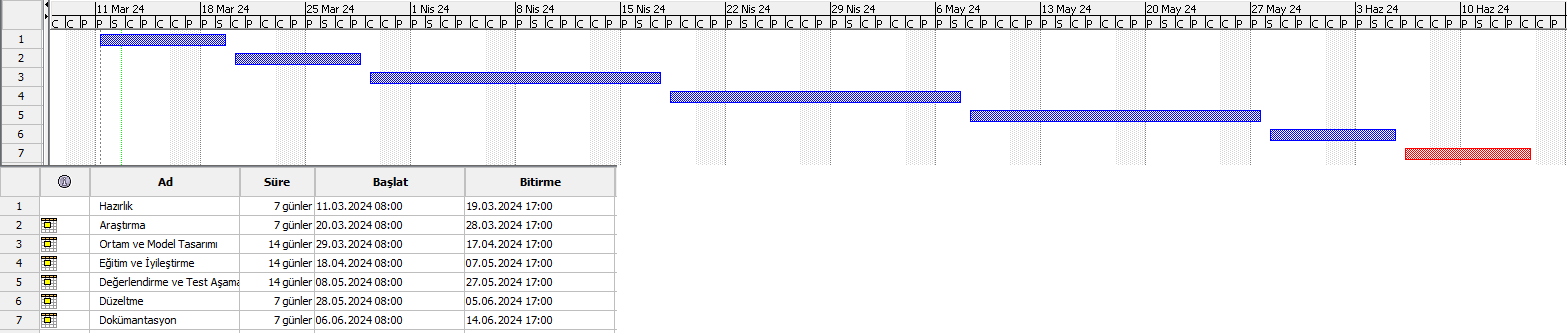
\includegraphics[angle=360,width=1.6\textwidth]{ganchartt.png}\centering % Resim dosyasının adını ve uzantısını belirtin
  \caption{Gantt Chart}
  \label{fig:resim_etiketi}
\end{figure}
    % Yana çevirmek istediğiniz içerik buraya gelir
\end{landscape}

\clearpage

\section{Beklenen Sonuçlar}
\rule{\textwidth}{0.5pt}
\subsection{Hayatta Kalma Becerilerinin Gelişmesi}
Projenin en temel beklenen sonuçlarından biri, yapay zekanın belirlenen ortamda hayatta kalmayı öğrenmesidir. Derin öğrenme algoritmaları, AI'nın ortama uyum sağlamasını ve tehlikeleri önceden tahmin etmesini sağlayarak hayatta kalma becerilerini geliştirecektir.
\subsection{Esneklik ve Adaptasyon Yeteneği}
AI'nın öğrendiği hayatta kalma stratejileri, değişen ortam koşullarına uyum sağlamak için esnek olacaktır. Bu, AI'nın çeşitli senaryolara ve farklı koşullara hızlı bir şekilde uyum sağlayabilme yeteneğini içerecektir.
\subsection{Optimize Edilmiş Karar Alma Yeteneği}
Pekiştirmeli öğrenme algoritmaları, AI'nın belirlenen hedeflere ulaşmak için en uygun kararları almasını sağlayacaktır. Bu, kaynakları verimli kullanma, riskleri minimize etme ve belirlenen hedeflere ulaşma konularında optimize edilmiş karar alma yeteneği anlamına gelir.
\subsection{Belirsizlik ve Karmaşıklıkla Başa Çıkma Yeteneği}
Proje, AI'nın belirsizlik ve karmaşıklıkla başa çıkma yeteneğini geliştirecek ve öngörülemeyen durumlarla nasıl başa çıkacağını öğretecektir. Bu, AI'nın değişen ortam koşullarında tutarlı bir şekilde performans göstermesini sağlayacaktır.

\subsection{Transfer Öğrenme ve Genelleme Yeteneği}
AI, öğrendiği hayatta kalma stratejilerini farklı ortamlara ve senaryolara transfer edebilecek ve bu stratejileri genelleştirebilecektir. Bu, AI'nın bir ortamda öğrendiklerini başka bir ortama veya görev üzerine uygulayabilme yeteneği anlamına gelir.
\subsection{Sürdürülebilir Performans ve Güvenilirlik}
Eğitilen modelin sürdürülebilir performansı ve güvenilirliği, projenin önemli sonuçlarından biridir. AI'nın belirlenen görevleri başarıyla yerine getirebilmesi ve sürekli olarak istikrarlı bir şekilde performans gösterebilmesi beklenmektedir.
\subsection{Endüstriyel ve Ticari Uygulamalar}
Elde edilen sonuçlar, çeşitli endüstriyel ve ticari uygulamalarda kullanılabilir. Örneğin, robotik sistemlerde, otonom araçlarda, oyun geliştirme alanında ve daha birçok alanda AI'nın hayatta kalma becerilerini geliştirmek için kullanılabilir.
\newpage
\bibliographystyle{ieeetr}
\bibliography{referance}

\end{document}
